\chapter{Evaluation}
\label{sec:eval}

\todo{how realistic is the simulation?}
\todo{which properties can be modelled well, which can't?}
\section{Testing with Joystick}


In order to evaluate, at an early stage, how flyable and responsivee to external commands the VREP Quadcopter was, and how reliable the communication link between the V-REP and the Ivy-Bus system is, a Hardware-in-the-loop (HIL) set-up was build. \ref{fig:finkenHIL} shows the HIL set-up, consisting of a joystick, which is attached on the Ivy-Bus and controls the V-REP Quadcopter.


\begin{figure}[h!]
 \begin{center}
  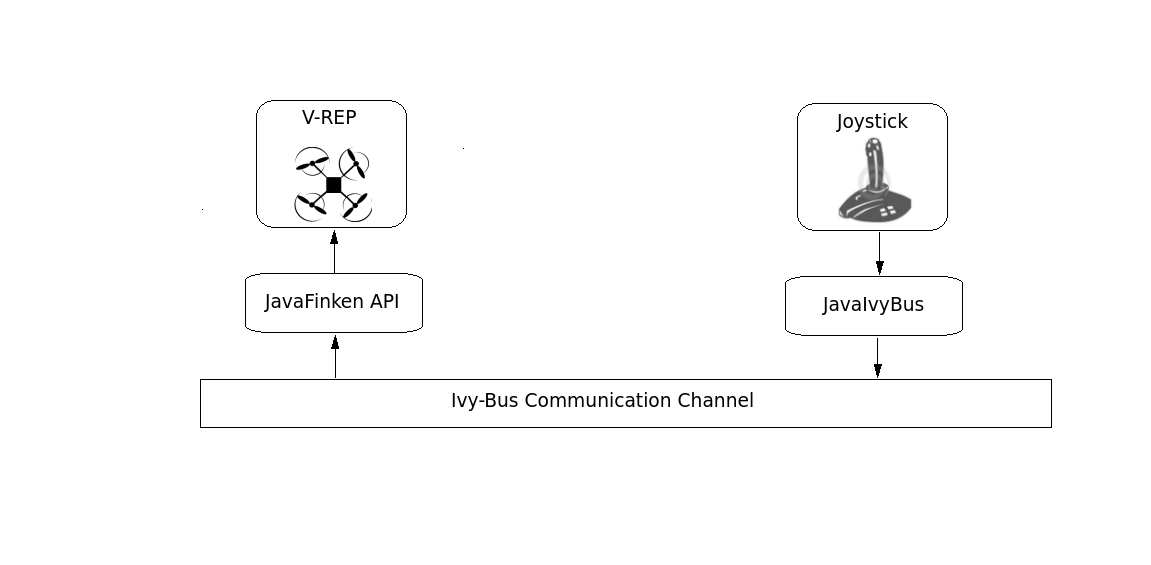
\includegraphics[scale=0.5]{FinkenHIL.png}
 \end{center}
  \caption{Finken Hardware-in-the-loop\label{fig:finkenHIL}}
\end{figure}

The HIL evaluation was implemented as a separate project - \textit{JavaFinkenSimHil}. It uses the Java external library \href{https://java.net/projects/jinput}{JInput} for reading the inputs from the joystick. The already created \textit{JavaIvyBus} module, which was discussed in \ref{sec:ivyBusImplementation}, is used to connect the Joystick to the Ivy-Bus. \\
The \textit{Joystick} class has as a local variable the class \textit{JoystickBusNode}, which extends the abstract \textit{AbsIvyBusNode}, thus being able to communicate on the common Ivy-Bus network. \\
The \textit{Joystick} class polls the data from the Joystick device at 50 Mhz and sends them to the \textit{JoystickBusNode}, which on the other hand encapsulates the data in 
a FINKEN\_ROTORCRAFT\_FP message and publishes it on the bus. \\ 
The FINKEN\_ROTORCRAFT\_FP is the message that the real Quadcopter uses to publish its pitch, yaw and roll angles. Since the Joystick fakes the real Quadcopter, the JavaFinkenApp receives the message as if coming from the real one, thus not even a single line of code had to be changed in the JavaFinkenApp, in order to use the HIL evaluation. \\

As a result of the evaluation we came to the following conclusions:

\begin{itemize}
\item{The controlling of the Quadcopter was very precise and accurate. We ware able to make any manoeuvre and flight path as desired. \\ When flying with the Joystick, one can get a real feeling
of the Quadcopter flight dynamics and behaviour}.

\item{We experienced challenges with keeping the Quadcopter at a level height, using the throttle levers of the Joystick. It turned out, that keeping a level height was a matter of eye-hand coordination. \\
Even the slightest change to the thrust when hovering resulted in a strong accelaration in $z$-axis. Even if this behaviour corresponds to the real quadcopter, we identified it as a problem, as the hover thrust of the real quadcopter changes during flight time with the battery voltage. As a result, we decided to tune the throttle response of the virtual Quadcopter with a logistic curve as described in \ref{equ:logistic}}.

\end{itemize}

\section{Speed}


\todo{communication delay}
\begin{itemize}

\item{mean delta t between sent messages, compare with the configured message frequency}
\item{ run this with two or multiple quadrocopter}
\item{latency of JAVA link}
\end{itemize}


\todo{vrep simulation speed}
\todo{run vrep on the 10core computer in the lab, look at mean execution time}
\todo{add multiple copter}


\section{Accuracy}
\begin{figure}
\begin{center}
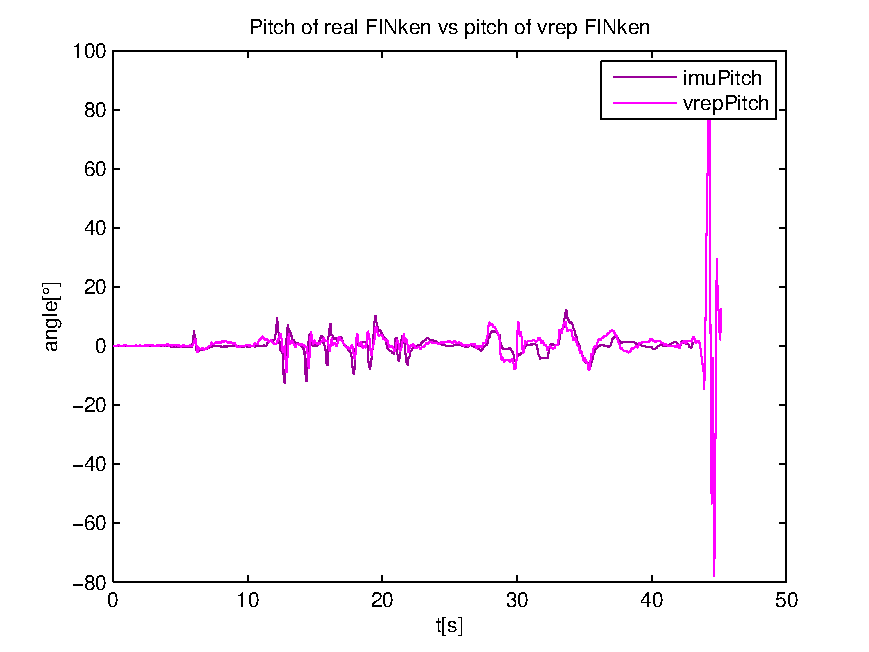
\includegraphics[width=\textwidth]{pitch}
\caption{Euler angles of simulated FINken and real FINken}
\label{pic:pitchResponse}
\end{center}
\end{figure}
\begin{figure}
\begin{center}
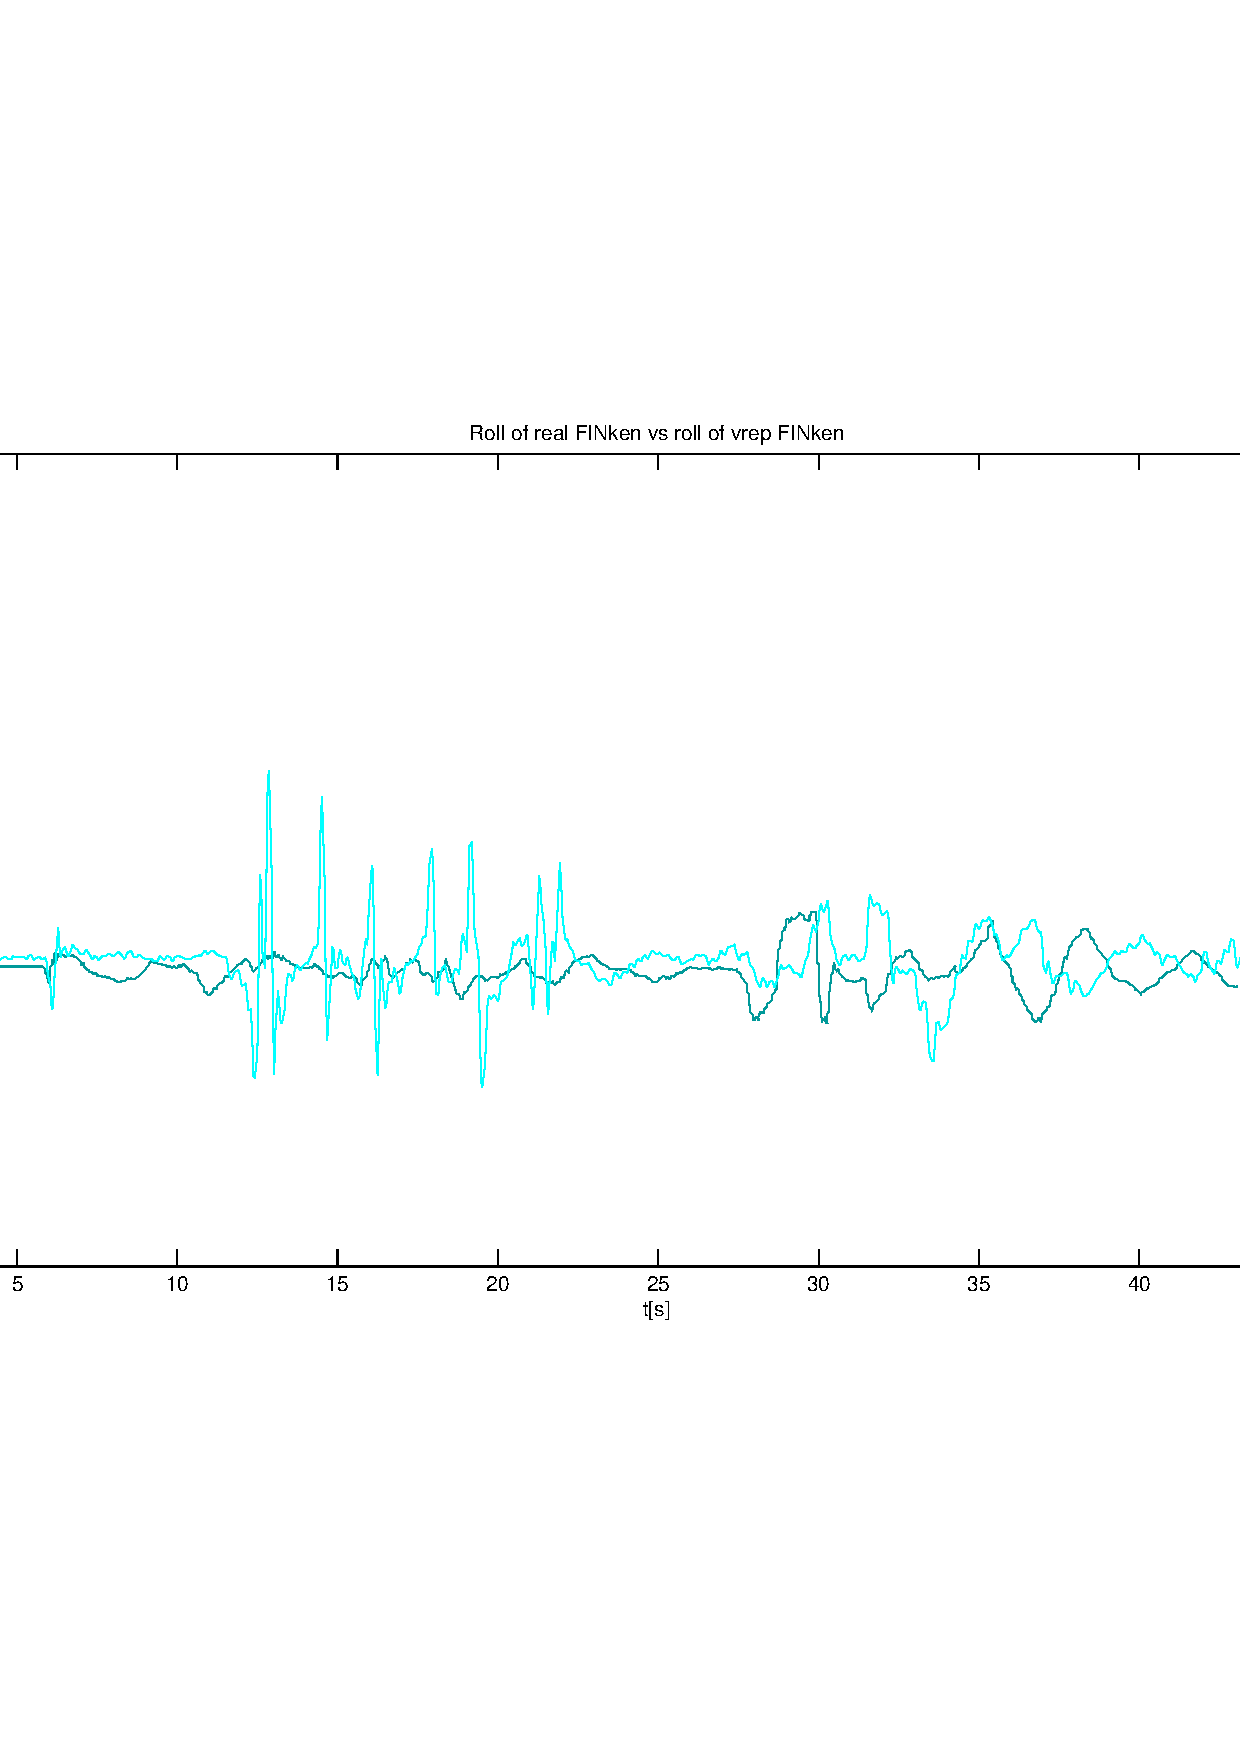
\includegraphics[width=\textwidth]{roll}
\caption{Euler angles of simulated FINken and real FINken}
\label{pic:rollResponse}
\end{center}
\end{figure}
\todo{explanation for roll spikes: vreps internal handling of shapes; maybe copter and "IMU" are not moved at the same time? }
\todo{filter values? }
\begin{itemize}
\item{plot graph of euler angles}
\item{highlight start of drift, other interesting elements?}
\item{plot difference between graphs}
\end{itemize}

Eventually we wanted to evaluate to what extend the path of the flying quadrocopter matches the path of the simulated quadcopter. V-REP provides an easy way to plot the two dimensional position of the quadrocopter and draw the flying path, but our real quadrocopter does not have a positioning system and its position estimation is not possible.\\ In order to estimate the position we have used the MEDUSA localization system developed in our faculty [add reference to the paper]. The system calculates the two dimensional position of a mobile robot moving in a rectangular arena, using eight proximity sensors and a gyroscope. It uses the yaw angle of the robot and the distances to the walls from the proximity sensors to calculate a set of possible positions, where the quadrocopter could be. Then it moves through all possible points and calculates the distances, that the proximity sensors should read at that particular point and angle of rotation. Comparing the real readings from the quadrocopter proximity sensors and the calculated distances, a probability function is calculated, that indicates the probability that the real quadrocopter is situated at the particular point. The point with the highest probability is chosen for the quadcopter position.\\
The MEDUSA positioning system turned out to be an easy and fast way to get an estimation of the position, since our quadcopter has four ultrasound sensors, positioned at 90 degrees from each other, and a gyroscope, which provides the angle of rotation. The fact, that the original positioning system uses eight distance sensors was not disturbing, since it is possible to estimate the position even with two sensors. But a higher number of sensors provides more fault-tolerance to the system and more accuracy. It was also not necessary to implement the algorithm in the firmware of the quadcopter. We used the log file, that the Paparazzi software uses to write the sensor data and fetch the sensor readings from there using a Matlab script. Only a minor changes ware required in the configuration of the sensor numbers, the sensors maximum range and the size of the arena.\\
On \ref{fig:matlabPosEstimation} you can see the calculated possible positions and the quadcopter positioned at the point with the highest possibility value. The lines represent the ultrasound sensors and the length of the lines depict the maximum sensor range. The red fractions of the lines show the actual distance measured by the sensor. 

\begin{figure}[h!]
 \begin{center}
  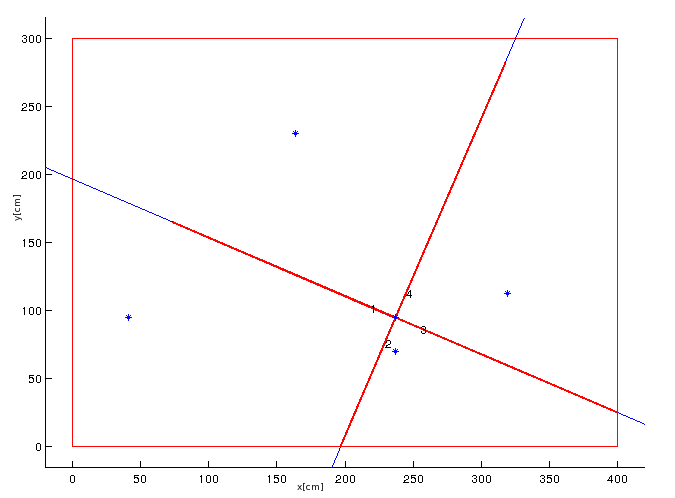
\includegraphics[scale=0.7]{MatlabPositionEstimation.png}
 \end{center}
  \caption{position estimation\label{fig:matlabPosEstimation}}
\end{figure}

The positioning system relies on accurate sensor readings to provide a precise position estimation. Our gyroscope provides noisy estimation of the yaw angle and the distance sensors are also quite noisy. Since our quadcopter is equipped with just four distance sensors, the localization system cannot tolerate the noise as good as with eight sensors. For this reasons an accurate position estimation could not be expected, but it should provide some reference estimation of the flying path. On \ref{fig:matlabPosPath} you can see the results of the position estimation. Each position has been marked with a blue star, so that we can see where the quadcopter has been. It is not possible to show the actual flying path as a function of time, but it shows which parts of the arena had been occupied by the quadcopter during the flight. \ref{fig:vrepPosPath} shows the flight path of the simulated quadcopter in the V-REP. As in \ref{fig:matlabPosPath} it does not shows the trajectory as a function of time, but just the occupied positions during the flight. The x and y axes of the plot show the V-REP scene arena and the small rectangle represents the flight arena.

\begin{figure}[h!]
 \begin{center}
  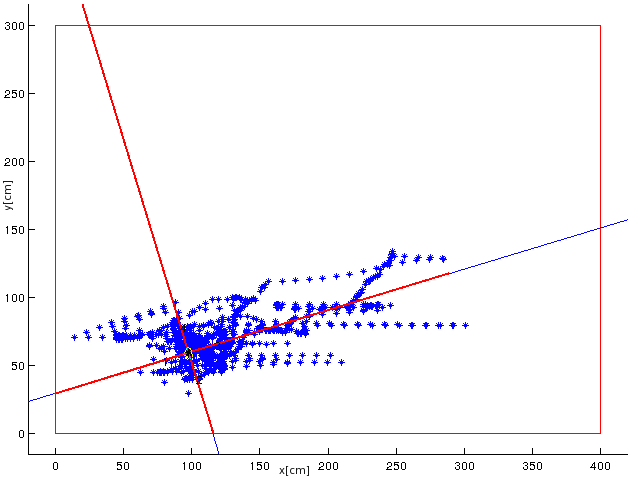
\includegraphics[scale=0.7]{MatlabPositionPath.png}
 \end{center}
  \caption{Estimated flight path\label{fig:matlabPosPath}}
\end{figure}

\begin{figure}[h!]
 \begin{center}
  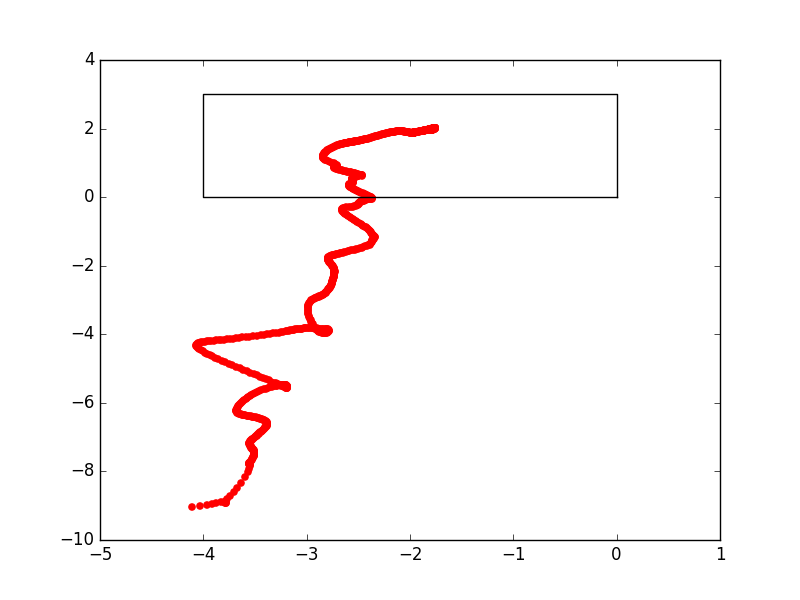
\includegraphics[scale=0.7]{vrepPath.png}
 \end{center}
  \caption{V-REP flight path\label{fig:vrepPosPath}}
\end{figure}

The estimated positions on \ref{fig:matlabPosPath} are very scattered, due to the fact that the localization system cannot estimate the position with a big accuracy. In the worst case, as a correct position was assumed one of the calculated possible points, which was far away from the previous estimated position. This creates a big jumps in the path, which does not coincide with the real flight path. The scattered plot and the jumps are caused by the noisy sensor measurements. A couple of attempts to filter the sensor readings ware made, but the plot still looked scattered to a significant extend. Also a Kalman Filter was implemented to eliminate the big jumps between the current and previous quadcopter positions, but the results ware still not satisfying.\\
On the other hand \ref{fig:vrepPosPath} shows a clear flying path, because the position is not estimated, but taken directly from the V-REP environment.


\begin{itemize}
\item{stability}
\item{time that both copter stay inside the arena}
\item{what happens when copter start to drift away?}
\item{maybe show angular movement plot at this time to find explanation there}
\end{itemize}

